\documentclass[../WiSe22ANA3.tex]{subfiles}
\begin{document}
	\lesson{1}{di 17 jan 2023 08:15}{Galilei- und Lorentz-Transformation} 
		\section{Transformationen}
			\noindent Eine bisher bekannte Transformation zwischen Basen ist die \emph{Galilei-Transformation}. 
			\begin{info}[Gaililei-Transformation]
				Eine Funktion $f:\R\times\Abb{\R}{\R^3}\to\R^4$ nennen wir \emph{Galilei-Transformation}, wenn 
				$$(t,\gamma)\mapsto\fdef{\begin{cases}
					\stern{\gamma}{i}{t}-\stern{\gamma'}{i}{t}\cdot t & i\in[3] \\
					t \sonst
				\end{cases}}{i\in[4]}.$$
			\end{info}
			\noindent Dann ist mithilfe der Galilei-Transformation ein transformierter Raumzeitvektor 
			$$\mcG(t,r)=\\
				\fdef{\begin{cases}
				\stern{r}{i}{t}-\stern{r'}{i}{t}\cdot t & i\in[3] \\
				t \sonst
				\end{cases}}{i\in[4]},$$
			wobei wir $\Mengenschriftdesign{Raumzeitvektor}_{\tilde r}(t,\tilde r(t)):=f(t,r)$ feststellen. Es wird derselbe Ort beschrieben, jedoch aus der Sicht einer anderen Basis. 
			\begin{Aufgabe}
				\nr Vollziehe die Schritte mathematisch nach. Prüfe, ob die Definition des Raumzeitvektors optimal gelungen ist. 
			\end{Aufgabe}
			\noindent Neu ist die sogenannte \Lorentz-Transformation. Sie ergibt sich aus der Überlegung und Forderung einer konstanten Lichtgeschwindigkeit $c_0$, wie wir sie bisher unkommentiert notiert haben. 
				
			\begin{info}[Spezielle Lorentztransformation]
				Seien die Systeme $\Sigma_1,\Sigma_2$ Basen des $K$-Vektorraums $\mcM$ und beschreibe $\gamma_1,\gamma_2\in C^{1}(\R,\mcM)$ die Orte von $\Sigma_1,\Sigma_2$ mit der Bedingung $\gamma_1(0)=\gamma_2(0)$. 
				
				Habe $\Sigma_2$ die zu $\Sigma_1$ relative Geschwindigkeit $(\gamma_1-\gamma_2)'(t):=v\cdot\underline e_1$, dann ist ein Ereignis an $r_{\Sigma_1}\in C^1(\R,\mcM)$ aus der Sicht von $\Sigma_2$ transformierbar mit 
				$$L_{(s,1)}:\clfdef{\R\times\mcM}{\mcM}{(v,x)}{
				\begin{pmatrix}
					k(v)\cdot (x_1+\cmath v/c_0\cdot x_4) \\
					x_2 \\
					x_3 \\
					k(v)\cdot (x_4-\cmath v/c_0\cdot x_1)
				\end{pmatrix}}.$$
			\end{info}
			\begin{Aufgabe}
				\nr Betrachte noch einmal genau $\stern{L_s\circ (\gamma_1-r)}{4}{t}$. Kann man auch einen Zusammenhang zu $\stern{\gamma_1-r}{4}{t}=\cmath c_0t$ herstellen?
				
				\nr Sei $\gamma_1:=\fdef{(0,0,0,\cmath c_0 t)}{t\in\R}$ und $\gamma_2:=\fdef{(v\cdot t,0,0,\cmath c_0t}{t\in\R}$. Berechne $(L_s\circ(\gamma_1-r))(t)$ für $r:=\fdef{(1,1,1,\cmath c_0t)}{t\in\R}$. 
				
				\nr Zeige $\lim_{v\to 0}(L_s\circ (\gamma_1-r))(t)=\mcG(t,\gamma_1)$ für $\mcG$ als Galilei-Transformation. 
				
				\nr Finde die Darstellungsmatrix von $\Maus{L}{s,1}$ nachdem du gezeigt hast, daß Linearität vorliegt. Zeige weiter $M(\Maus{L}{s,1},\underline v,\underline w)$ ist orthogonal. 
			\end{Aufgabe}
			Zur Veranschaulichung der Situation hilft ein Gedankenexperiment mit folgender Visualisierung:
			\begin{figure}[H]
				\centering
				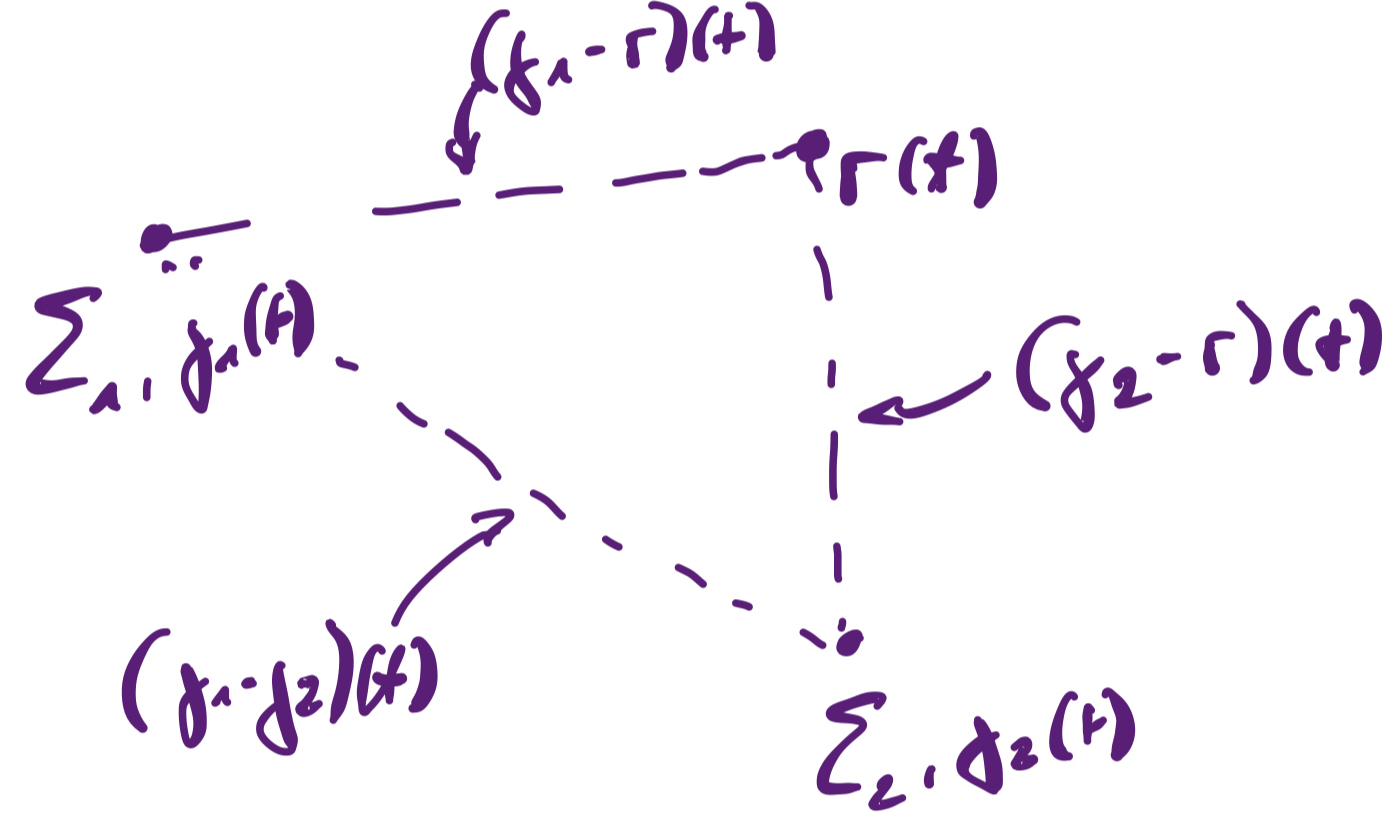
\includegraphics[width=5cm]{Bilddateien/IMG_8130.jpg}
				\caption{Darstellung der Situation im Anschauungsraum.}
			\end{figure}
			Eine wichtige Bedingung der Lorentz-Transformation war die konstante Lichtgeschwindigkeit. Unter den im Satz angebrachten Bedingungen folgt für die Norm
			\begin{align*}
				\dabs{(L_s\circ (\gamma_1-r))(t)}{P}:=&\sqrt{g(P)((L_s\circ (\gamma_1-r))(t),(L_s\circ (\gamma_1-r))(t))} \\
				=&\sum_{i\in[4]}\stern{L_s\circ (\gamma_1-r)}{i}{t}^2 \\
				=&\sum_{i\in[3]}\stern{L_s\circ (\gamma_1-r)}{i}{t}^2-c_0^2\cdot k(v)^2\cdot\nbra{t-\frac{v\cdot\stern{\gamma-r}{3}{t}}{c_0^2}}^2.
			\end{align*}
			Nach Definition und Wahl der Situation können wir nun den ersten Summanden schreiben als
			\begin{multline*}
				\sum_{i\in[3]}\stern{L_s\circ (\gamma_1-r)}{i}{t}^2 \\
				=\stern{L_s\circ (\gamma_1-r)}{1}{t}^2+\stern{\gamma_1-r}{2}{t}+\stern{\gamma_1-r}{3}{t}.
			\end{multline*}
			\begin{Aufgabe}
				\nr Zeige die Gleichung $\sqrt{g(P)((L_s\circ (\gamma_1-r))(t),(L_s\circ (\gamma_1-r))(t))}=\sum_{i\in[4]}\stern{L_s\circ (\gamma_1-r)}{i}{t}^2$. 
			\end{Aufgabe}
			
				
			\begin{info}[Relative Systemaussicht]
				Seien $\Sigma_1,\Sigma_2$ zwei Systeme der Weltlinien $\gamma_{\Sigma_1},\gamma_{\Sigma_2}\in C^1(\R,\mcM)$. Dann beschreiben wir die \emph{relative Aussicht} von $\Sigma_1$ ruhend auf $\sigma_2$ bewegend \emph{bezüglich der Attribute} $\gamma'_{\Sigma_2}$ als Auswertung 
				$$\Aussicht{\Sigma_1}{\Sigma_2}{\gamma_{\Sigma_2}}:=\nbra{\mcL\circ\nbra{\dabs{\gamma'_{\Sigma_2}}{(P,\mcM)},\gamma'_{\Sigma_2}}}.$$
			\end{info}
			Als Graphik veranschaulichen wir uns die Konstruktion wiefolgt.
			\begin{figure}[H]
				\centering
				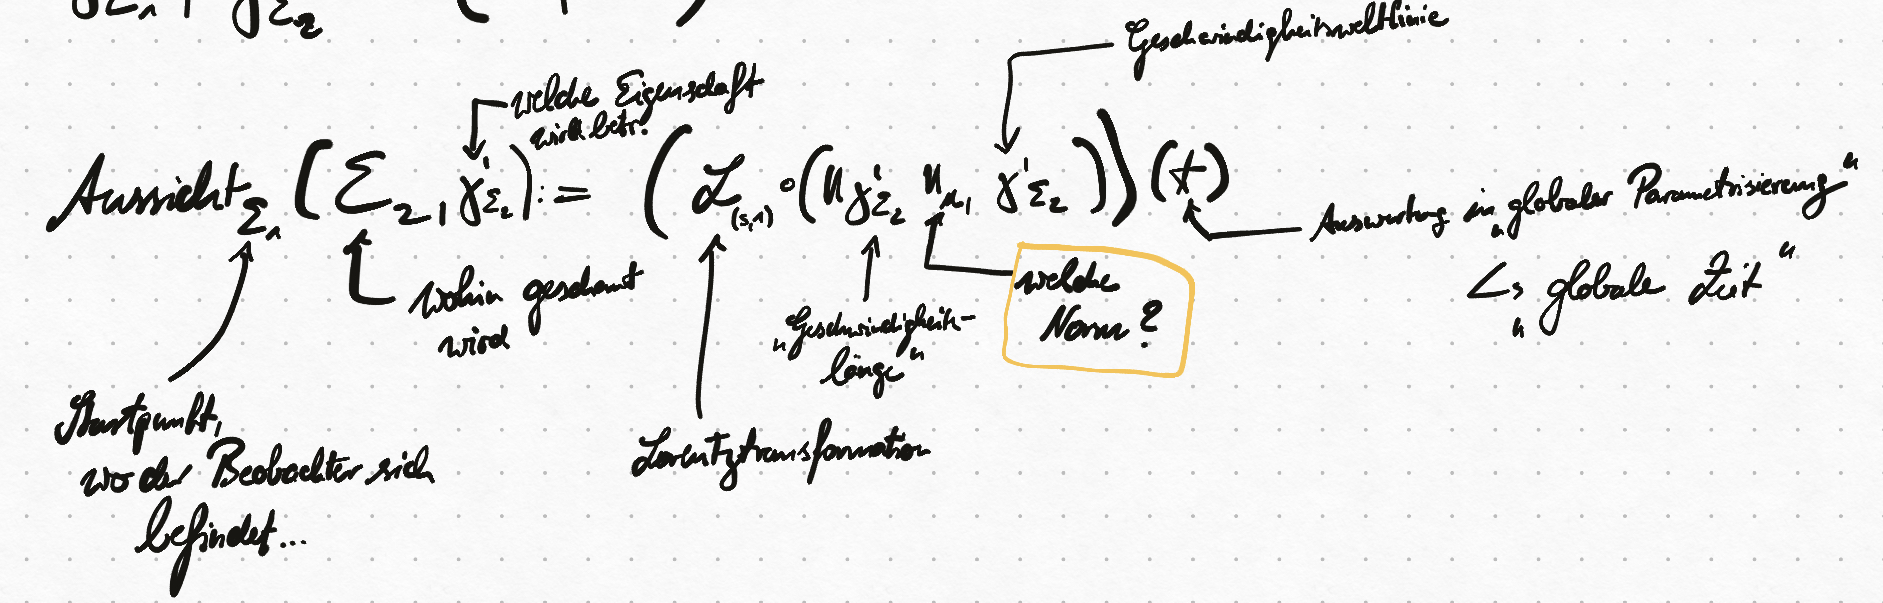
\includegraphics[width=7cm]{Bilddateien/IMG_5C89688377FE-1.jpeg}
			\end{figure}
			Hierduch geben wir der Lorentz-Transformation eine Anschauung. 
			
		\section{Maxwell Gleichungen}
			Ziel des Kapitels ist eine kompakte Schreibweise der Maxwell Gleichung. Hierzu betrachten wir zunächst den bekannten Satz.
			\begin{info}[Die Maxwell-Gleichungen]
				Die \Maxwell Gleichungen der Elektrodynamik lauten
				\begin{align*}
					&\div\vec{E}=\frac{\rho}{\epsilon_0} &&\div\vec{D}=\rho \\
					&\rot\vec{E}=-\pdiff{\vec{B}}{t}{}{} &&\rot\vec{H}=\vec{j}+\pdiff{\vec{D}}{t}{}{}.
				\end{align*}
			\end{info}
			Aus den Gleichungen (i) und (ii) können wir folgern, daß $\vec E$ und $\vec B$ aus Potential- und Rotatorfeld konstruierbar sind, sodaß folgt
			\begin{align*}
				&\vec B=\rot\vec A &&\vec E=-\grad\varphi+\pdiff{A}{t}{}{}.
			\end{align*}
			Setzen wir diese in Gleichungen (iii) und (iv) ein, so erhalten wir mit $\vec D=\epsilon\epsilon_0\vec E$ und $\epsilon=1_\R$ die Beziehung
			$$\div\nbra{-\grad\varphi-\pdiff{A}{t}{}{}}=\rho/\epsilon_0\Longleftrightarrow\laplace\varphi+\pdiff{\div A}{t}{}{}=-\rho/\epsilon_0.$$
			Mit Gleichung (iv) haben wir schließlich 
			$$\rot(\vec B)-\mu_0\cdot\pdiff{\vec D}{t}{}{}=\vec j\cdot\mu_0$$
			mit $\vec H=\vec B/\mu_0$ und schließlich durch Linearität der Ableitung mit den obigen Definitionen
			$$\rot(\rot \vec A)+\mu_0\epsilon_0\cdot\pdiff{(\grad\phi)}{t}{}{}=\vec j\cdot\mu_0.$$
			\begin{Aufgabe}
				\nr Rechne die Umformungen nach. 
			\end{Aufgabe}
			
			\subsection*{Die Eichtoleranz}
				Betrachten wir nun eine Änderung der Funktionen $\vec B:=\fdef{\rot\vec A}{A\in C^0(\R^3,\R^3)}$ und $\vec E:=\fdef{-\grad\varphi}{\varphi\in C^0(\R^3,\R)}$, dann ergibt sich
				$$\diff{B}{H}{A}{}\approx B(A+H)-B(A)\approx \rot(A+H).\rot A$$
				und mit Linearität von rot schließlich $\diff{B}{H}{A}{}\approx\rot A$, sodaß wir sagen können $\vec B$ ist \emph{stabil unter kleinen Änderungen}. Da wir $H=\grad\mch$ und analog $\mch=\pdiff{h}{t}{}{	}$ für das Analogon von $\vec E$ wählen können ($H,\mch$ beliebig), wählen wir die folgende vorteilhafte Form.
				\begin{info}[Lorenz Eichung]
					Als \emph{Lorenz Eichung} verstehen wir eine Funktion $\chi\in C^2(\R^d,\R)$, welche das DGP 
					$$\Phi(t,(u(t),u'(t),u''(t))):=\grad u(t)-\frac{1}{c_0^2}\pdiff{\chi}{t}{t}{2}=0$$
					löst, also $\chi\in\Lsng{\Phi}$. 
				\end{info}
				\begin{Aufgabe}
					\nr[EFeldLsng] Verfolge den analogen Weg zu $\vec B$ für $\vec E$, indem du die Definition verwendest und die Änderung $\diff{\vec E}{\mch}{\varphi}{}$ bestimmst. 
				\end{Aufgabe} 
				Durch die Wahl der Eichung ist uns garantiert, daß die Lorenz Bedingung
				$$\div\vec A+\frac{1}{c_0^2}\pdiff{\varphi}{t}{t}{}=0_\R$$
				in einem beliebigen Inertialsystem eingehalten wird. Mit der am Anfang durchgeführten umformulierung der Gleichung (iii) des Maxwell Satzes haben wir  
				$$\laplace\varphi+\pdiff{\nbra{-\frac{1}{c_0^2}\pdiff{\varphi}{t}{t}{}}}{t}{t}{}=-\frac{\rho}{\epsilon_0}.$$
				\InfoblockDAlembertOperatorDef
				Mithilfe der Abkürzung können wir nun formulieren
				$$\dal\vec A=-\mu_0 j.$$
				\begin{Aufgabe}
					\nr Zeige die Kovarianz der Gleichung, wobei wir \emph{kovariant} als $\alpha\in\dual{V}$ definieren... (Größen ändern sich durch Transformation).
				\end{Aufgabe}
				
			\subsection*{Änderung bei Inertialsystemwechsel}
				Wir behalten hierbei wieder im Hinterkopf, daß ein \emph{Inertialsystemwechsel} nichts als ein \emph{Basiswechsel} ist, wobei die Start- und Zielbasis bestimmte Kräfteanforderungen auf Körper erfüllen sollen. Sei $\Sigma_1$ ein stationäres und $\Sigma_2$ ein mit $v(t)=(0,0,v_0,\cmath c_0)$ relativ bewegtes System. Dann lautet die Lorentz-Transformationsmatrix
				$$L=\begin{pmatrix}
					1 & 0 & 0 & 0 \\
					0 & 1 & 0 & 0 \\
					0 & 0 & k(v_0) & k(v_0)\cdot\cmath v/c_0 \\
					0 & 0 & k(v_0)\cdot\cmath v/c_0 & k(v_0)
				\end{pmatrix}$$
				
\end{document}